% Created by tikzDevice version 0.12.6 on 2024-06-24 18:27:32
% !TEX encoding = UTF-8 Unicode
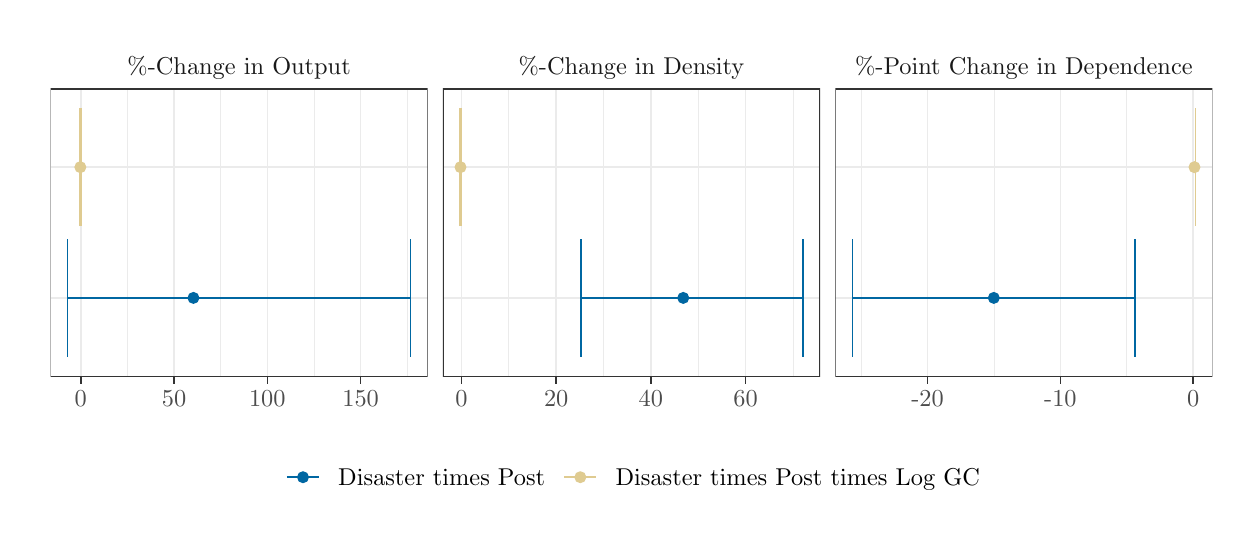
\begin{tikzpicture}[x=1pt,y=1pt]
\definecolor{fillColor}{RGB}{255,255,255}
\path[use as bounding box,fill=fillColor,fill opacity=0.00] (0,0) rectangle (433.62,180.67);
\begin{scope}
\path[clip] (  0.00,  0.00) rectangle (433.62,180.67);
\definecolor{drawColor}{RGB}{255,255,255}
\definecolor{fillColor}{RGB}{255,255,255}

\path[draw=drawColor,line width= 0.6pt,line join=round,line cap=round,fill=fillColor] (  0.00,  0.00) rectangle (433.62,180.68);
\end{scope}
\begin{scope}
\path[clip] (  8.25, 54.68) rectangle (144.54,158.60);
\definecolor{fillColor}{RGB}{255,255,255}

\path[fill=fillColor] (  8.25, 54.68) rectangle (144.54,158.60);
\definecolor{drawColor}{gray}{0.92}

\path[draw=drawColor,line width= 0.3pt,line join=round] ( 36.05, 54.68) --
	( 36.05,158.60);

\path[draw=drawColor,line width= 0.3pt,line join=round] ( 69.75, 54.68) --
	( 69.75,158.60);

\path[draw=drawColor,line width= 0.3pt,line join=round] (103.45, 54.68) --
	(103.45,158.60);

\path[draw=drawColor,line width= 0.3pt,line join=round] (137.15, 54.68) --
	(137.15,158.60);

\path[draw=drawColor,line width= 0.6pt,line join=round] (  8.25, 83.02) --
	(144.54, 83.02);

\path[draw=drawColor,line width= 0.6pt,line join=round] (  8.25,130.26) --
	(144.54,130.26);

\path[draw=drawColor,line width= 0.6pt,line join=round] ( 19.20, 54.68) --
	( 19.20,158.60);

\path[draw=drawColor,line width= 0.6pt,line join=round] ( 52.90, 54.68) --
	( 52.90,158.60);

\path[draw=drawColor,line width= 0.6pt,line join=round] ( 86.60, 54.68) --
	( 86.60,158.60);

\path[draw=drawColor,line width= 0.6pt,line join=round] (120.30, 54.68) --
	(120.30,158.60);
\definecolor{drawColor}{RGB}{0,103,162}
\definecolor{fillColor}{RGB}{0,103,162}

\path[draw=drawColor,line width= 0.4pt,line join=round,line cap=round,fill=fillColor] ( 59.90, 83.02) circle (  1.96);
\definecolor{drawColor}{RGB}{223,203,145}
\definecolor{fillColor}{RGB}{223,203,145}

\path[draw=drawColor,line width= 0.4pt,line join=round,line cap=round,fill=fillColor] ( 19.03,130.26) circle (  1.96);
\definecolor{drawColor}{RGB}{0,103,162}

\path[draw=drawColor,line width= 0.6pt,line join=round] (138.34, 61.76) --
	(138.34,104.28);

\path[draw=drawColor,line width= 0.6pt,line join=round] (138.34, 83.02) --
	( 14.45, 83.02);

\path[draw=drawColor,line width= 0.6pt,line join=round] ( 14.45, 61.76) --
	( 14.45,104.28);
\definecolor{drawColor}{RGB}{223,203,145}

\path[draw=drawColor,line width= 0.6pt,line join=round] ( 19.26,109.00) --
	( 19.26,151.52);

\path[draw=drawColor,line width= 0.6pt,line join=round] ( 19.26,130.26) --
	( 18.81,130.26);

\path[draw=drawColor,line width= 0.6pt,line join=round] ( 18.81,109.00) --
	( 18.81,151.52);
\definecolor{drawColor}{gray}{0.20}

\path[draw=drawColor,line width= 0.6pt,line join=round,line cap=round] (  8.25, 54.68) rectangle (144.54,158.60);
\end{scope}
\begin{scope}
\path[clip] (150.04, 54.68) rectangle (286.33,158.60);
\definecolor{fillColor}{RGB}{255,255,255}

\path[fill=fillColor] (150.04, 54.68) rectangle (286.33,158.60);
\definecolor{drawColor}{gray}{0.92}

\path[draw=drawColor,line width= 0.3pt,line join=round] (173.88, 54.68) --
	(173.88,158.60);

\path[draw=drawColor,line width= 0.3pt,line join=round] (208.10, 54.68) --
	(208.10,158.60);

\path[draw=drawColor,line width= 0.3pt,line join=round] (242.32, 54.68) --
	(242.32,158.60);

\path[draw=drawColor,line width= 0.3pt,line join=round] (276.54, 54.68) --
	(276.54,158.60);

\path[draw=drawColor,line width= 0.6pt,line join=round] (150.04, 83.02) --
	(286.33, 83.02);

\path[draw=drawColor,line width= 0.6pt,line join=round] (150.04,130.26) --
	(286.33,130.26);

\path[draw=drawColor,line width= 0.6pt,line join=round] (156.77, 54.68) --
	(156.77,158.60);

\path[draw=drawColor,line width= 0.6pt,line join=round] (190.99, 54.68) --
	(190.99,158.60);

\path[draw=drawColor,line width= 0.6pt,line join=round] (225.21, 54.68) --
	(225.21,158.60);

\path[draw=drawColor,line width= 0.6pt,line join=round] (259.43, 54.68) --
	(259.43,158.60);
\definecolor{drawColor}{RGB}{0,103,162}
\definecolor{fillColor}{RGB}{0,103,162}

\path[draw=drawColor,line width= 0.4pt,line join=round,line cap=round,fill=fillColor] (236.89, 83.02) circle (  1.96);
\definecolor{drawColor}{RGB}{223,203,145}
\definecolor{fillColor}{RGB}{223,203,145}

\path[draw=drawColor,line width= 0.4pt,line join=round,line cap=round,fill=fillColor] (156.40,130.26) circle (  1.96);
\definecolor{drawColor}{RGB}{0,103,162}

\path[draw=drawColor,line width= 0.6pt,line join=round] (280.13, 61.76) --
	(280.13,104.28);

\path[draw=drawColor,line width= 0.6pt,line join=round] (280.13, 83.02) --
	(200.00, 83.02);

\path[draw=drawColor,line width= 0.6pt,line join=round] (200.00, 61.76) --
	(200.00,104.28);
\definecolor{drawColor}{RGB}{223,203,145}

\path[draw=drawColor,line width= 0.6pt,line join=round] (156.56,109.00) --
	(156.56,151.52);

\path[draw=drawColor,line width= 0.6pt,line join=round] (156.56,130.26) --
	(156.24,130.26);

\path[draw=drawColor,line width= 0.6pt,line join=round] (156.24,109.00) --
	(156.24,151.52);
\definecolor{drawColor}{gray}{0.20}

\path[draw=drawColor,line width= 0.6pt,line join=round,line cap=round] (150.04, 54.68) rectangle (286.33,158.60);
\end{scope}
\begin{scope}
\path[clip] (291.83, 54.68) rectangle (428.12,158.60);
\definecolor{fillColor}{RGB}{255,255,255}

\path[fill=fillColor] (291.83, 54.68) rectangle (428.12,158.60);
\definecolor{drawColor}{gray}{0.92}

\path[draw=drawColor,line width= 0.3pt,line join=round] (301.16, 54.68) --
	(301.16,158.60);

\path[draw=drawColor,line width= 0.3pt,line join=round] (349.18, 54.68) --
	(349.18,158.60);

\path[draw=drawColor,line width= 0.3pt,line join=round] (397.19, 54.68) --
	(397.19,158.60);

\path[draw=drawColor,line width= 0.6pt,line join=round] (291.83, 83.02) --
	(428.12, 83.02);

\path[draw=drawColor,line width= 0.6pt,line join=round] (291.83,130.26) --
	(428.12,130.26);

\path[draw=drawColor,line width= 0.6pt,line join=round] (325.17, 54.68) --
	(325.17,158.60);

\path[draw=drawColor,line width= 0.6pt,line join=round] (373.18, 54.68) --
	(373.18,158.60);

\path[draw=drawColor,line width= 0.6pt,line join=round] (421.19, 54.68) --
	(421.19,158.60);
\definecolor{drawColor}{RGB}{0,103,162}
\definecolor{fillColor}{RGB}{0,103,162}

\path[draw=drawColor,line width= 0.4pt,line join=round,line cap=round,fill=fillColor] (349.11, 83.02) circle (  1.96);
\definecolor{drawColor}{RGB}{223,203,145}
\definecolor{fillColor}{RGB}{223,203,145}

\path[draw=drawColor,line width= 0.4pt,line join=round,line cap=round,fill=fillColor] (421.62,130.26) circle (  1.96);
\definecolor{drawColor}{RGB}{0,103,162}

\path[draw=drawColor,line width= 0.6pt,line join=round] (400.20, 61.76) --
	(400.20,104.28);

\path[draw=drawColor,line width= 0.6pt,line join=round] (400.20, 83.02) --
	(298.02, 83.02);

\path[draw=drawColor,line width= 0.6pt,line join=round] (298.02, 61.76) --
	(298.02,104.28);
\definecolor{drawColor}{RGB}{223,203,145}

\path[draw=drawColor,line width= 0.6pt,line join=round] (421.93,109.00) --
	(421.93,151.52);
\definecolor{drawColor}{gray}{0.20}

\path[draw=drawColor,line width= 0.6pt,line join=round,line cap=round] (291.83, 54.68) rectangle (428.12,158.60);
\end{scope}
\begin{scope}
\path[clip] (  8.25,158.60) rectangle (144.54,175.17);
\definecolor{drawColor}{gray}{0.10}

\node[text=drawColor,anchor=base,inner sep=0pt, outer sep=0pt, scale=  0.88] at ( 76.40,163.86) {\%-Change in Output};
\end{scope}
\begin{scope}
\path[clip] (150.04,158.60) rectangle (286.33,175.17);
\definecolor{drawColor}{gray}{0.10}

\node[text=drawColor,anchor=base,inner sep=0pt, outer sep=0pt, scale=  0.88] at (218.18,163.86) {\%-Change in Density};
\end{scope}
\begin{scope}
\path[clip] (291.83,158.60) rectangle (428.12,175.17);
\definecolor{drawColor}{gray}{0.10}

\node[text=drawColor,anchor=base,inner sep=0pt, outer sep=0pt, scale=  0.88] at (359.98,163.86) {\%-Point Change in Dependence};
\end{scope}
\begin{scope}
\path[clip] (  0.00,  0.00) rectangle (433.62,180.67);
\definecolor{drawColor}{gray}{0.20}

\path[draw=drawColor,line width= 0.6pt,line join=round] ( 19.20, 51.93) --
	( 19.20, 54.68);

\path[draw=drawColor,line width= 0.6pt,line join=round] ( 52.90, 51.93) --
	( 52.90, 54.68);

\path[draw=drawColor,line width= 0.6pt,line join=round] ( 86.60, 51.93) --
	( 86.60, 54.68);

\path[draw=drawColor,line width= 0.6pt,line join=round] (120.30, 51.93) --
	(120.30, 54.68);
\end{scope}
\begin{scope}
\path[clip] (  0.00,  0.00) rectangle (433.62,180.67);
\definecolor{drawColor}{gray}{0.30}

\node[text=drawColor,anchor=base,inner sep=0pt, outer sep=0pt, scale=  0.88] at ( 19.20, 43.66) {0};

\node[text=drawColor,anchor=base,inner sep=0pt, outer sep=0pt, scale=  0.88] at ( 52.90, 43.66) {50};

\node[text=drawColor,anchor=base,inner sep=0pt, outer sep=0pt, scale=  0.88] at ( 86.60, 43.66) {100};

\node[text=drawColor,anchor=base,inner sep=0pt, outer sep=0pt, scale=  0.88] at (120.30, 43.66) {150};
\end{scope}
\begin{scope}
\path[clip] (  0.00,  0.00) rectangle (433.62,180.67);
\definecolor{drawColor}{gray}{0.20}

\path[draw=drawColor,line width= 0.6pt,line join=round] (156.77, 51.93) --
	(156.77, 54.68);

\path[draw=drawColor,line width= 0.6pt,line join=round] (190.99, 51.93) --
	(190.99, 54.68);

\path[draw=drawColor,line width= 0.6pt,line join=round] (225.21, 51.93) --
	(225.21, 54.68);

\path[draw=drawColor,line width= 0.6pt,line join=round] (259.43, 51.93) --
	(259.43, 54.68);
\end{scope}
\begin{scope}
\path[clip] (  0.00,  0.00) rectangle (433.62,180.67);
\definecolor{drawColor}{gray}{0.30}

\node[text=drawColor,anchor=base,inner sep=0pt, outer sep=0pt, scale=  0.88] at (156.77, 43.66) {0};

\node[text=drawColor,anchor=base,inner sep=0pt, outer sep=0pt, scale=  0.88] at (190.99, 43.66) {20};

\node[text=drawColor,anchor=base,inner sep=0pt, outer sep=0pt, scale=  0.88] at (225.21, 43.66) {40};

\node[text=drawColor,anchor=base,inner sep=0pt, outer sep=0pt, scale=  0.88] at (259.43, 43.66) {60};
\end{scope}
\begin{scope}
\path[clip] (  0.00,  0.00) rectangle (433.62,180.67);
\definecolor{drawColor}{gray}{0.20}

\path[draw=drawColor,line width= 0.6pt,line join=round] (325.17, 51.93) --
	(325.17, 54.68);

\path[draw=drawColor,line width= 0.6pt,line join=round] (373.18, 51.93) --
	(373.18, 54.68);

\path[draw=drawColor,line width= 0.6pt,line join=round] (421.19, 51.93) --
	(421.19, 54.68);
\end{scope}
\begin{scope}
\path[clip] (  0.00,  0.00) rectangle (433.62,180.67);
\definecolor{drawColor}{gray}{0.30}

\node[text=drawColor,anchor=base,inner sep=0pt, outer sep=0pt, scale=  0.88] at (325.17, 43.66) {-20};

\node[text=drawColor,anchor=base,inner sep=0pt, outer sep=0pt, scale=  0.88] at (373.18, 43.66) {-10};

\node[text=drawColor,anchor=base,inner sep=0pt, outer sep=0pt, scale=  0.88] at (421.19, 43.66) {0};
\end{scope}
\begin{scope}
\path[clip] (  0.00,  0.00) rectangle (433.62,180.67);
\definecolor{fillColor}{RGB}{255,255,255}

\path[fill=fillColor] ( 86.76,  5.50) rectangle (349.61, 30.95);
\end{scope}
\begin{scope}
\path[clip] (  0.00,  0.00) rectangle (433.62,180.67);
\definecolor{fillColor}{RGB}{255,255,255}

\path[fill=fillColor] ( 92.26, 11.00) rectangle (106.71, 25.45);
\end{scope}
\begin{scope}
\path[clip] (  0.00,  0.00) rectangle (433.62,180.67);
\definecolor{drawColor}{RGB}{0,103,162}
\definecolor{fillColor}{RGB}{0,103,162}

\path[draw=drawColor,line width= 0.4pt,line join=round,line cap=round,fill=fillColor] ( 99.49, 18.23) circle (  1.96);
\end{scope}
\begin{scope}
\path[clip] (  0.00,  0.00) rectangle (433.62,180.67);
\definecolor{drawColor}{RGB}{0,103,162}

\path[draw=drawColor,line width= 0.6pt,line join=round] ( 93.70, 18.23) -- (105.27, 18.23);
\end{scope}
\begin{scope}
\path[clip] (  0.00,  0.00) rectangle (433.62,180.67);
\definecolor{fillColor}{RGB}{255,255,255}

\path[fill=fillColor] (192.47, 11.00) rectangle (206.92, 25.45);
\end{scope}
\begin{scope}
\path[clip] (  0.00,  0.00) rectangle (433.62,180.67);
\definecolor{drawColor}{RGB}{223,203,145}
\definecolor{fillColor}{RGB}{223,203,145}

\path[draw=drawColor,line width= 0.4pt,line join=round,line cap=round,fill=fillColor] (199.70, 18.23) circle (  1.96);
\end{scope}
\begin{scope}
\path[clip] (  0.00,  0.00) rectangle (433.62,180.67);
\definecolor{drawColor}{RGB}{223,203,145}

\path[draw=drawColor,line width= 0.6pt,line join=round] (193.92, 18.23) -- (205.48, 18.23);
\end{scope}
\begin{scope}
\path[clip] (  0.00,  0.00) rectangle (433.62,180.67);
\definecolor{drawColor}{RGB}{0,0,0}

\node[text=drawColor,anchor=base west,inner sep=0pt, outer sep=0pt, scale=  0.88] at (112.21, 15.20) {Disaster times Post};
\end{scope}
\begin{scope}
\path[clip] (  0.00,  0.00) rectangle (433.62,180.67);
\definecolor{drawColor}{RGB}{0,0,0}

\node[text=drawColor,anchor=base west,inner sep=0pt, outer sep=0pt, scale=  0.88] at (212.42, 15.20) {Disaster times Post times Log GC};
\end{scope}
\end{tikzpicture}